\chapter{Physics II}
This compendium is based on the course notes of MIT 8.02 2004 \url{https://web.mit.edu/8.02t/www/802TEAL3D/visualizations/coursenotes/index.htm} and the lectures of MIT 8.02 by Professor Walter Lewin in 2002. The video lectures can be viewed on YouTube from Lectures by ``Walter Lewin. They will make you \ensuremath\varheartsuit~Physics.'' with the playlist name ``8.02x - MIT Physics II: Electricity and Magnetism''
All credits go to Dr. Sen-ben Liao, Dr. Peter Dourmashkin, and Professor John W. Belcher at MIT for the lecture notes and Professor Walter Lewin for the inspiring lectures. I can not guarantee the accuracy of this compendium and that it is a correct interpretation of the material and explanation provided by the lecture notes and lectures. Thus, for accurate information refer to the material that this compendium is based on. If a mistake is in the compendium it is most likely my fault and not the fault of the material in which this compendium is based on.


\section{Introduction}
\subsection{Electric Charges}
%\section{Electric Charges and Forces and Coulomb's Law - Polarization}
An atom comprises positively charged protons, neutrally charged neutrons, and negatively charged electron.
An atom or molecule can have a neutral, positive or negative electric charge. A negatively charged atom or molecule is called a \textit{negative ion}, meaning to a surplus of electrons compared to protons.
A positively charged atom or molecule is called a \textit{positive ion}.
The nucleus, the protons and neutrons or the atom, is significantly larger than an electron, a proton with a size of $10^{-15}\SI{}{\meter}$ is roughly 1000 times larger than an electron with a size of $10^{-18}\SI{}{\meter}$.
For a hydrogen atom the lower energy state has the most probable distance, using Bohr Radius, of approximately $10^{-11}\SI{}{\meter}$ from the nucleus, which is 10000 times further than the size of the hydrogens' proton.

An intuitive way of thinking why same changed ions repel each other and why opposite charged ions attracted each other is to think about a room where we have loud and talkative people who want someone to listen to them, i.e., negative ions, and quiet, shy listeners, positive ions. When a loud and talkative person is approached by another loud and talkative person they talk over each other and neither gets want they want and find it physically uncomfortable to be near each other, they naturally repel each other. Likewise, if two quite people talk to each other they find it awkward and physically uncomfortable to be close each other. However, if there are a quite, shy listener and a loud talkative person they have found there mach.

Conductors allows electrons to flow ``freely'', there is always some resistance. Continuing with our metaphor we can think of it as a channel where the voice of the loud and talkative person can travel far and reach the quite, shy listener. And non-conductors are like a wall where the voice does not travel through.

\subsection{Polarization}

If we have a positive charge object like we see with the rod in Figure~\ref{fig:charged-rod} placed next to a conductive object like we see with the cloud shaped object next to the rod, the conductive object will have a negative and a positive charged side. Only $10^{13}$ of electrons that was originally on the left side might have moves to the right side.

\begin{figure}[H]
\centering
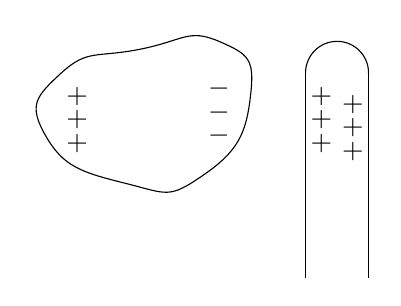
\begin{tikzpicture}

  % Shape of the object
  \path[draw=black]
    plot[smooth cycle, tension=1] coordinates {
      (0,0.4) (1,0.5) (1.4,-0.2)
      (0.8,-1.2) (-0.2,-1.3)
      (-1.2,-0.7) (-1,0.1)
    };

	\node at (-0.8,-0.2) {$+$};
	\node at (-0.8,-0.5) {$+$};
	\node at (-0.8,-0.8) {$+$};

	\node at (1.0,-0.1) {$-$};
	\node at (1.0,-0.4) {$-$};
	\node at (1.0,-0.7) {$-$};


	\draw (2.1,0.1) -- (2.1,-2.5);
	\draw (2.9,0.1) -- (2.9,-2.5);
	\draw (2.1,0.1) arc[start angle=180, end angle=0, radius=4mm];

	\node at (2.3,-0.2) {$+$};
	\node at (2.3,-0.5) {$+$};
	\node at (2.3,-0.8) {$+$};

	\node at (2.7,-0.3) {$+$};
	\node at (2.7,-0.6) {$+$};
	\node at (2.7,-0.9) {$+$};

\end{tikzpicture}
  \caption{Positively charged rod next to some conductive object}
  \label{fig:charged-rod}
\end{figure}

What happens in Figure~\ref{fig:charged-rod} mostly due to induction where the atoms become polarized, i.e., the electron spends more time on one side than the other.
\begin{figure}[H]
\centering
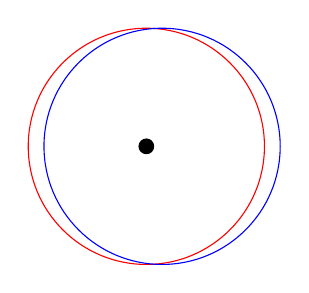
\begin{tikzpicture}

  \fill (0,0) circle (1mm);
  \draw[red] (0,0) circle (15mm);
  \draw[blue] (0.2,0) circle (15mm);

	\end{tikzpicture}
  \caption{Polarized atom is shown with the blue circle and red is non polarized.}
  \label{fig:polarized-atom}
\end{figure}

\begin{figure}[H]
     \centering
     \begin{subfigure}[b]{0.4\textwidth}
         \centering
         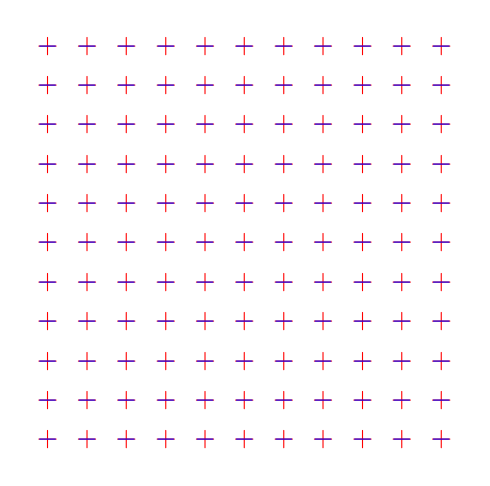
\begin{tikzpicture}

          \foreach \y in {0,1,...,10}
          {
            \foreach \x in {0,1,...,10}
            {
              \pgfmathtruncatemacro{\xnegpos}{0.5*\x + 0.02};
              \pgfmathtruncatemacro{\ynegpos}{0.5*\y + 0.02};
              \node[red] at (0.5*\x,0.5*\y) {$+$};
              \node[blue] at (0.5*\x,0.5*\y) {$-$};
            }
          }

         \end{tikzpicture}
         \caption{No induction, where $-$ is over $+$.}
         \label{fig:y equals x}
     \end{subfigure}
     \hfill
     \begin{subfigure}[b]{0.4\textwidth}
         \centering
          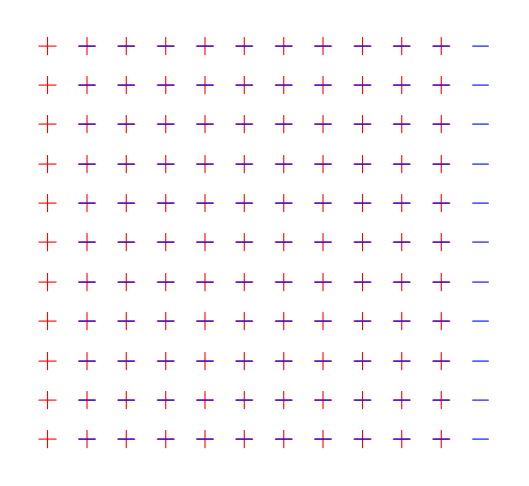
\begin{tikzpicture}


          \foreach \y in {0,...,10}
          {
            \foreach \x in {0,...,10}
            {
              \node[red] at (0.5*\x,0.5*\y) {$+$};
            }
            \foreach \x in {1,...,11}
            {
              \node[blue] at (0.5*\x,0.5*\y) {$-$};
            }
          }


         \end{tikzpicture}
         \caption{Induction, where $-$ is shifted to the right.}
         \label{fig:three sin x}
     \end{subfigure}
        \caption{No induction compared to induction.}
        \label{fig:three graphs}
\end{figure}

\section{Coulomb's Law}
\subsection{Electric Forces and Coulomb's Law}
%31:50 Coulomb's Law 
%40:00 what holds the world together, the autom scale the neculer force, then the electric force and on the size of planets and galixies it is the gravitational force. why
Coulomb's law describes the force resulted by two charged points $q_1$ and $q_2$, separated by a distance $r$ in vacuum.
\begin{equation}
  \vec{\boldsymbol{F}}_{12} = k_e \frac{q_1q_2}{r^2}\hat{\boldsymbol{r}}
\end{equation}
where $k_e$ is Coulomb's constant. The director $\hat{\boldsymbol{r}}$ is the unit vector directed from $q_1$ and $q_2$ defined as $\hat{\boldsymbol{r}}=\vec{\boldsymbol{r}}/r$. The direction of the force is determined by the sign of $q_1q_2\hat{\boldsymbol{r}}$, $(+)(+)=$ the same direction of $\hat{\boldsymbol{r}}$, $(-)(-)=$ same direction, $(+)(-)=$ opposite direction, and $(-)(+)=$ opposite direction.
See Figure~\ref{fig:coulomb-illustration} for the illustration of Coulomb's law.

\begin{figure}[H]
\centering
     \centering
     \begin{subfigure}[b]{0.45\textwidth}
         \centering
  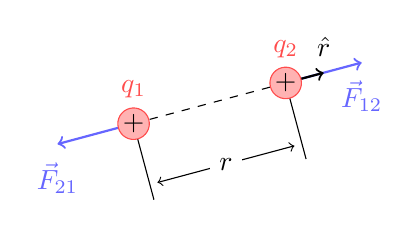
\begin{tikzpicture}

	\begin{scope}[rotate=15] 
    \draw[thick, blue!60, ->] (0,0) -- (-1,0) node[below=1mm] {$\vec{\boldsymbol{F}}_{21}$};  
    \draw[thick, blue!60, ->] (2,0) -- (3,0) node[below=1mm] {$\vec{\boldsymbol{F}}_{12}$}; 
    \draw[thick, ->] (2,0) -- (2.5,0) node[above=0.8mm] {$\hat{\boldsymbol{r}}$}; 

    \draw[dashed] (0,0) -- (2,0); 
    \draw (0,0) -- (0,-1);
    \draw (2,0) -- (2,-1);
    \draw[<->](0.1,-0.8)--(1.9,-0.8) node[midway,fill=white]{$r$};

    \filldraw[color=red!70, fill=red!30] (0,0) circle (2mm) node[above=2mm] {$q_1$};
    \node at (0,0) {$+$}; 
    \filldraw[color=red!70, fill=red!30] (2,0) circle (2mm) node[above=2mm] {$q_2$};
    \node at (2,0) {$+$}; 
  \end{scope}

	\end{tikzpicture}
       \caption{Repel (P - P).}
  \label{fig:coulomb-illustration-repel-p-p}
  \end{subfigure}
     \hfill
  \begin{subfigure}[b]{0.45\textwidth}
    \centering
  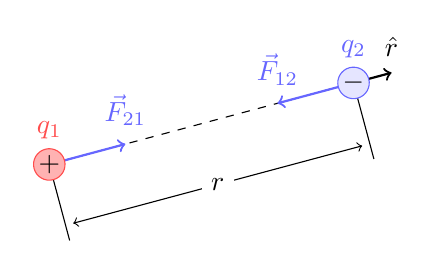
\begin{tikzpicture}

	\begin{scope}[rotate=15] 
    \draw[dashed] (0,0) -- (4,0); 
    \draw (0,0) -- (0,-1);
    \draw (4,0) -- (4,-1);
    \draw[<->](0.1,-0.8)--(3.9,-0.8) node[midway,fill=white]{$r$};
    \draw[thick, ->] (4,0) -- (4.5,0) node[above=0.8mm] {$\hat{\boldsymbol{r}}$}; 

    \draw[thick, blue!60, ->] (0,0) -- (1,0) node[above=1mm] {$\vec{\boldsymbol{F}}_{21}$};  
    \draw[thick, blue!60, ->] (4,0) -- (3,0) node[above=1mm] {$\vec{\boldsymbol{F}}_{12}$}; 


    \filldraw[color=red!70, fill=red!30] (0,0) circle (2mm) node[above=2mm] {$q_1$};
    \node at (0,0) {$+$}; 
    \filldraw[color=blue!60, fill=blue!10] (4,0) circle (2mm) node[above=2mm] {$q_2$};
    \node at (4,0) {$-$}; 
  \end{scope}

	\end{tikzpicture}
  \caption{Attracted (P - N).}
  \label{fig:coulomb-illustration-attracted-p-n}
  \end{subfigure}
\begin{subfigure}[b]{0.45\textwidth}
    \centering
  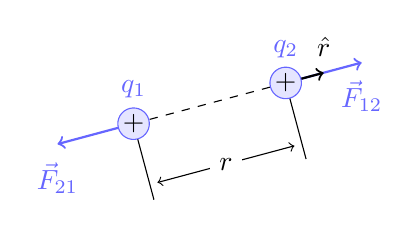
\begin{tikzpicture}

	\begin{scope}[rotate=15] 
    \draw[thick, blue!60, ->] (0,0) -- (-1,0) node[below=1mm] {$\vec{\boldsymbol{F}}_{21}$};  
    \draw[thick, blue!60, ->] (2,0) -- (3,0) node[below=1mm] {$\vec{\boldsymbol{F}}_{12}$}; 
    \draw[thick, ->] (2,0) -- (2.5,0) node[above=0.8mm] {$\hat{\boldsymbol{r}}$}; 

    \draw[dashed] (0,0) -- (2,0); 
    \draw (0,0) -- (0,-1);
    \draw (2,0) -- (2,-1);
    \draw[<->](0.1,-0.8)--(1.9,-0.8) node[midway,fill=white]{$r$};

    \filldraw[color=blue!60, fill=blue!10] (0,0) circle (2mm) node[above=2mm] {$q_1$};
    \node at (0,0) {$+$}; 
    \filldraw[color=blue!60, fill=blue!10] (2,0) circle (2mm) node[above=2mm] {$q_2$};
    \node at (2,0) {$+$}; 
  \end{scope}

	\end{tikzpicture}
  \caption{Repel (N - N).}
  \label{fig:coulomb-illustration-repel-n-n}
  \end{subfigure}
     \hfill
  \begin{subfigure}[b]{0.45\textwidth}
    \centering
  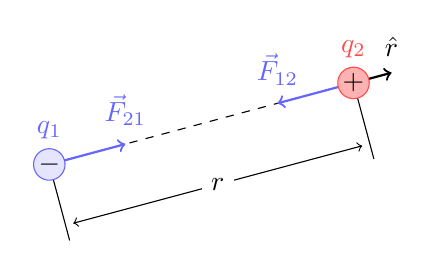
\begin{tikzpicture}

	\begin{scope}[rotate=15] 
    \draw[dashed] (0,0) -- (4,0); 
    \draw (0,0) -- (0,-1);
    \draw (4,0) -- (4,-1);
    \draw[<->](0.1,-0.8)--(3.9,-0.8) node[midway,fill=white]{$r$};
    \draw[thick, ->] (4,0) -- (4.5,0) node[above=0.8mm] {$\hat{\boldsymbol{r}}$}; 

    \draw[thick, blue!60, ->] (0,0) -- (1,0) node[above=1mm] {$\vec{\boldsymbol{F}}_{21}$};  
    \draw[thick, blue!60, ->] (4,0) -- (3,0) node[above=1mm] {$\vec{\boldsymbol{F}}_{12}$}; 


    \filldraw[color=blue!60, fill=blue!10] (0,0) circle (2mm) node[above=2mm] {$q_1$};
    \node at (0,0) {$-$}; 
    \filldraw[color=red!70, fill=red!30] (4,0) circle (2mm) node[above=2mm] {$q_2$};
    \node at (4,0) {$+$}; 
  \end{scope}

	\end{tikzpicture}
  \caption{Attracted (N - P).}
  \label{fig:coulomb-illustration-attracted-n-p}
  \end{subfigure}

  \caption{Illustration of Coulomb's Law.}
  \label{fig:coulomb-illustration}

\end{figure}


Coulomb's constant $k_e$ is defined as:
\begin{equation*}
  k_e = \frac{1}{4\pi\varepsilon_0} = \SI[per-mode = fraction]{8.9875e9}{\newton\meter\squared\per\coulomb\squared}
\end{equation*}
where $\varepsilon_0$ is the \textbf{Vacuum Permittivity}, also known as the
\textbf{Electric Constant} or the \textbf{Permittivity of Free Space}, i.e., a
measure of how much resistance the vacuum of empty space puts up against an
electric field.
\begin{equation*}
  \varepsilon_0 = \SI[per-mode = fraction]{8.85e-12}{\coulomb\squared\per\newton\meter\squared}
\end{equation*}


\section{Principle of Superposition}
Coulomb's laws applies to a pair of charged points and when there are more than
two charged points the net force on any charged point is the vector sum of all
forces exerted on it by the other changed points. 
\begin{equation*}
  \vec{\boldsymbol{F}}_{j} = \sum_{\substack{i=1 \\ j \neq i}}^{N} \vec{\boldsymbol{F}}_{ij}
\end{equation*}
where $\vec{\boldsymbol{F}}_{ij}$ denotes the force between charged point $i$ and $j$ for a system of $N$ charges.

\paragraph{Example:}
There are three charged points shown in Figure~\ref{fig:system-of-three-charges}. Find the force on charge $q_3$, when $q_1 = \SI{6.0e-6}{\coulomb}$, $q_2 = -q_1 = \SI{-6.0e-6}{\coulomb}$, $q_3 = \SI{3.0e-6}{\coulomb}$, and $\SI{2.0e-2}{\meter}$.

\begin{figure}[H]
\centering
\begin{tikzpicture}

  \draw (0,0) -- (0,4) node[above] {$y$} node[pos=0.4, left] {$a$};
  \draw (0,0) -- (4,0) node[right] {$x$};
  \draw[dashed] (0,0) -- (3,3) node[midway, below] {$\sqrt{2}a$};
  \draw[dashed] (3,3) -- (5,3);
  \draw (0,3) -- (3,3);
  \draw[dashed] (0.5,3) -- (1.5,4);
  \draw[dashed] (1.5,4) -- (4,4);
  \draw[thick] (1,0) arc[start angle=0, end angle=45, radius=10mm] node[midway, right] {$\theta$};
  \draw[thick, dashed, -Stealth] (4.5,3) arc[start angle=45, end angle=110, radius=20mm] node[midway, right=3mm] {$\phi$};

  \draw[color=blue!60, very thick, -Stealth] (3,3) -- (0.5,3) node[below] {$\vec{\boldsymbol{F}}_{23}$};
  \draw[color=blue!60, very thick, -Stealth] (3,3) -- (1.5,4) node[above] {$\vec{\boldsymbol{F}}_{3}$};
  \draw[color=blue!60, very thick, -Stealth] (3,3) -- (4,4) node[above right] {$\vec{\boldsymbol{F}}_{13}$};

  \draw[very thick, -Stealth] (3,3) -- (3.5,3.5) node[below right=0.5mm] {$\hat{\boldsymbol{r}}_{13}$};;
  \draw[very thick, -Stealth] (3,3) -- (3.8,3) node[below] {$\hat{\boldsymbol{r}}_{23}$};

  \filldraw[color=red!70, fill=red!30] (0,0) circle (2mm) node[left=2mm] {$q_1$};
  \node at (0,0) {$+$}; 
  \filldraw[color=blue!60, fill=blue!10] (0,3) circle (2mm) node[left=2mm] {$q_2$};
  \node at (0,3) {$-$}; 
  \filldraw[color=red!70, fill=red!30] (3,3) circle (2mm) node[below=2mm] {$q_3$};
  \node at (3,3) {$+$}; 

\end{tikzpicture}
  \caption{A system of three charges.}
  \label{fig:system-of-three-charges}
\end{figure}


\subparagraph{Solution:}
Using the super position principle, the force on $q_3$ is
\begin{equation*}
  \vec{\boldsymbol{F}}_{3} = \vec{\boldsymbol{F}}_{13} +
  \vec{\boldsymbol{F}}_{23} = \frac{1}{4\pi\varepsilon_0} \left(
  \frac{q_1q_3}{r^2_{13}}\hat{\boldsymbol{r}}_{13} + \frac{q_2q_3}{r^2_{23}}\hat{\boldsymbol{r}}_{23} \right)
\end{equation*}
where the unit vector $\hat{\boldsymbol{r}}_{13}$ is 
\begin{equation*}
  \hat{\boldsymbol{r}}_{13} = \cos{\theta}\hat{\boldsymbol{i}} + \cos{\theta}\hat{\boldsymbol{j}} = \frac{\sqrt{2}}{2}(\hat{\boldsymbol{i}} + \hat{\boldsymbol{j}})
\end{equation*}
and $\hat{\boldsymbol{r}}_{23} = \hat{\boldsymbol{i}}$. Therefore, the total force is 
\begin{align*}
  \vec{\boldsymbol{F}}_{3} &= \frac{1}{4\pi\varepsilon_0} \left(
  \frac{q_1q_3}{r^2_{13}}\hat{\boldsymbol{r}}_{13} + \frac{q_2q_3}{r^2_{23}}\hat{\boldsymbol{r}}_{23} \right)
  = \frac{1}{4\pi\varepsilon_0} \left(
  \frac{q_1q_3}{(\sqrt{2}a)^2}\frac{\sqrt{2}}{2}(\hat{\boldsymbol{i}} + \hat{\boldsymbol{j}}) 
  + \frac{(-q_1)q_3}{a^2}\hat{\boldsymbol{i}} \right) \\
  &= \frac{1}{4\pi\varepsilon_0} \frac{q_1q_3}{a^2} \left(\left(
  \frac{\sqrt{2}}{4}-1\right)\hat{\boldsymbol{i}} + \frac{\sqrt{2}}{4}\hat{\boldsymbol{j}} \right) 
\end{align*}
The total force, i.e., the ``length'' of the vector, can be calculated by pythagorean theorem $c=\sqrt{a^2+b^2}$, which gives us
\begin{align*}
  \vec{\boldsymbol{F}}_{3} 
  &= \frac{1}{4\pi\varepsilon_0} \frac{q_1q_3}{a^2} \sqrt{\left(
  \frac{\sqrt{2}}{4}-1\right)^2 + \left(\frac{\sqrt{2}}{4}\right)^2 } \\
  &= \left(\SI[per-mode =
  fraction]{9.0e9}{\coulomb\squared\per\newton\meter\squared}\right)
  \frac{(\SI{6.0e-6}{\coulomb})(\SI{3.0e-6}{\coulomb})}{(\SI{2.0e-2}{\meter})^2}
  (0.74) = \SI{3.0}{\newton}
\end{align*}
The angle of the force from the x-axis is
\begin{equation*}
  \phi = \arctan{\left( \frac{F_{3,y}}{F_{3,x}} \right)}
  = \arctan{\left( \frac{\sqrt{2}/4}{-1+\sqrt{2}/4} \right)} = \SI{151.3}{\degree}
\end{equation*}



\section{Electric Fields}

An electric field $\vec{\boldsymbol{E}}$ is defined as the electric force per unit charge experienced by a small positive test charge placed at a point in space. The small positive test charge will be canceled out in the derivations so the actual value of test charge $q_0$ is not important, but we say that it is infinitesimally small.
\begin{equation*}
  \vec{\boldsymbol{E}} = \lim_{q_0\to0}\frac{\vec{\boldsymbol{F}}}{q_0}
\end{equation*}
And with Coulomb's law we get:
\begin{equation*}
  \vec{\boldsymbol{E}} = \frac{1}{4\pi\varepsilon_0}\frac{Qq_0}{q_0r^2}\hat{\boldsymbol{r}} 
  = \frac{1}{4\pi\varepsilon_0}\frac{Q}{r^2}\hat{\boldsymbol{r}} 
\end{equation*}
Where $Q$ is a stationary charge.

Now for all charges in a given space $q_i$, we can use the super position principle and get the following electric fields:
\begin{equation*}
  \vec{\boldsymbol{E}} = \sum_i\vec{\boldsymbol{E}}_i = \sum_i\frac{1}{4\pi\varepsilon_0}\frac{q_i}{r^2}\hat{\boldsymbol{r}} 
\end{equation*}


\subsection{Electric Fields Lines}
A convenient way of representing the electric fields are with electric field lines.
\begin{figure}[H]
\centering
  \begin{subfigure}[b]{0.45\textwidth}
    \centering
\begin{tikzpicture}[
    scale=0.80,
    attach arrow/.style args={#1}{
        decoration={
            markings,
            mark=at position 0 with {\pgfextra{%
                \pgfmathsetmacro{\tmpArrowTime}{\pgfkeysvalueof{/tikz/arc arrow/length}/(\pgfdecoratedpathlength)}%
                \xdef\tmpArrowTime{\tmpArrowTime}}},
            mark=at position {#1-3*\tmpArrowTime} with {\coordinate(@1);},
            mark=at position {#1-2*\tmpArrowTime} with {\coordinate(@2);},
            mark=at position {#1-1*\tmpArrowTime} with {\coordinate(@3);},
            mark=at position {#1+\tmpArrowTime/2} with {\coordinate(@4);
                \draw[-{Stealth[length=\pgfkeysvalueof{/tikz/arc arrow/length},bend]}]
                  plot[smooth] coordinates {(@1) (@2) (@3) (@4)};},
        },
        postaction=decorate,
    },
    attach arrow/.default=0.5,
    arc arrow/.cd, length/.initial=2mm,
]
\node[draw=red!70, fill=red!30, circle, minimum size=6mm] (Q) {+};

% Radial outward field lines
\foreach \a in {0,30,...,330} {
  \draw[red!70, thick, attach arrow={1/3}, attach arrow={2/3}] (Q) -- ++(\a:3);
}
\end{tikzpicture}
  \caption{}
  \label{fig:electric-field-line-for-positive}
  \end{subfigure}
     \hfill
  \begin{subfigure}[b]{0.45\textwidth}
    \centering
\begin{tikzpicture}[
    scale=0.80,
    attach arrow/.style args={#1}{
        decoration={
            markings,
            mark=at position 0 with {\pgfextra{%
                \pgfmathsetmacro{\tmpArrowTime}{\pgfkeysvalueof{/tikz/arc arrow/length}/(\pgfdecoratedpathlength)}%
                \xdef\tmpArrowTime{\tmpArrowTime}}},
            mark=at position {#1-3*\tmpArrowTime} with {\coordinate(@1);},
            mark=at position {#1-2*\tmpArrowTime} with {\coordinate(@2);},
            mark=at position {#1-1*\tmpArrowTime} with {\coordinate(@3);},
            mark=at position {#1+\tmpArrowTime/2} with {\coordinate(@4);
                \draw[-{Stealth[length=\pgfkeysvalueof{/tikz/arc arrow/length},bend]}]
                  plot[smooth] coordinates {(@1) (@2) (@3) (@4)};},
        },
        postaction=decorate,
    },
    attach arrow/.default=0.5,
    arc arrow/.cd, length/.initial=2mm,
]
\node[draw=blue!70, fill=blue!20, circle, minimum size=6mm] (Q) {$-$};

% Radial inward field lines
\foreach \a in {0,30,...,330} {
  \draw[red!70, thick, attach arrow={1/3}, attach arrow={2/3}] ++(\a:3) -- (Q);
}
\end{tikzpicture}
  \caption{}
  \label{fig:electric-field-line-negative}
  \end{subfigure}
  \caption{Field lines for (a) positive, radially outwards, and (b) negative charges, radially inwards.}
  \label{fig:electric-field-lines}
\end{figure}


\begin{figure}[H]
\centering
\begin{tikzpicture}[
    scale=1,
    attach arrow/.style={
        decoration={
            markings,
            mark=at position 0 with {\pgfextra{%
                \pgfmathsetmacro{\tmpArrowTime}{\pgfkeysvalueof{/tikz/arc arrow/length}/(\pgfdecoratedpathlength)}%
                \xdef\tmpArrowTime{\tmpArrowTime}}},
            mark=at position {#1-3*\tmpArrowTime} with {\coordinate(@1);},
            mark=at position {#1-2*\tmpArrowTime} with {\coordinate(@2);},
            mark=at position {#1-1*\tmpArrowTime} with {\coordinate(@3);},
            mark=at position {#1+\tmpArrowTime/2} with {\coordinate(@4);
                \draw[-{Stealth[length=\pgfkeysvalueof{/tikz/arc arrow/length},bend]}] plot[smooth]
                coordinates {(@1) (@2) (@3) (@4)};},
        },
        postaction=decorate,
    },
    attach arrow/.default=0.5,
    arc arrow/.cd,length/.initial=2mm,
    %nodes={circle,minimum size=2.4em,font=\bfseries\sffamily}
]
\path 
    node[draw=red!70, fill=red!30, circle, minimum size=6mm] (L){+} 
    (2.5,0) node[draw=blue!60, fill=blue!10, circle, minimum size=6mm] (R){--};
\foreach \X in {0,...,7}
 {\draw[red!70, thick, attach arrow] (L) 
 to[bend left={-70+\X*20},looseness=1.6] 
 (R);}
\foreach \X in {0,...,10}
 {\draw[red!70, thick,attach arrow/.list={1/3,2/3}] (L) to[bend left=16-4*\X] ++ (70+\X*22:3);
 \draw[red!70, thick,attach arrow/.list={1/3,2/3}] (R)+(180+70+\X*22:3) 
 to[bend right=16-4*\X] 
  (R);}
\end{tikzpicture}
  \caption{Field lines for an electric dipole.}
  \label{fig:electric-field-line-for-dipole}
\end{figure}


\subsection{Force Exerted on a Charged Particle in a Constant Electric Field}
Consider a charged particle $+q$ in an electric field formed by a positive and negative infinitely large source plates, as shown in Figure~\ref{fig:electric-field-of-source-plates}. 
\begin{figure}[H]
\centering
\begin{tikzpicture}
  \filldraw[color=red!70, fill=red!30] (0,3.5) rectangle (7,3.9);
  \filldraw[color=blue!60, fill=blue!10] (0,0) rectangle (7,0.4);
  \foreach \x in {0,...,6} {
	  \node at (\x+0.5,3.7) {$+$};
	  \node at (\x+0.5,0.2) {$-$};
  }
  \draw[<->] (0.2,0.4) -- (0.2,3.5) node[midway, fill=white] {$y$};
  \draw[red!70, ->] (6.8,3.5) -- (6.8,0.4) node[midway, right] {$\vec{\boldsymbol{E}}$};
  \draw[dashed] (3.5,3) -- (3.5,0.9);

  \filldraw[dotted, very thick, color=red!70, fill=white] (3.5,3) circle (2mm) node[right=2mm] {$q$};
  \filldraw[color=red!70, fill=red!30] (3.5,0.9) circle (2mm);

	\node at (2.5,2.8) {$\vec{\boldsymbol{V}}=\vec{\boldsymbol{0}}$};
  \draw[thick, -Stealth] (4,1.3) -- (4,0.6) node[midway, right] {$\vec{\boldsymbol{V}}$};

\end{tikzpicture}
  \caption{A charge $q$ moving in a constant electric field formed by two infinity large source plates.}
  \label{fig:electric-field-of-source-plates}
\end{figure}

The electric field between the source plates is $\vec{\boldsymbol{E}}=-E_y\hat{\boldsymbol{j}}$, with $E_y>0$. The charge $q$ will experience a downward force
\begin{equation*}
  \vec{\boldsymbol{F}}_e = q \vec{\boldsymbol{E}}
\end{equation*}

With Newton's Second Law $F=ma$, the net force will cause the charge to accelerate with an acceleration
\begin{equation*}
  \vec{\boldsymbol{a}} = \frac{\vec{\boldsymbol{F}}_e}{m} = \frac{q\vec{\boldsymbol{E}}}{m}
  = -\frac{qE_y}{m}\hat{\boldsymbol{j}}
\end{equation*}

Remember that the standard kinematics is described as $v_f^2=v_i^2+2ad$, where $v_f$ is the final velocity and $v_i$ is the initial velocity. The final velocity of the particle hitting the negative charged plate is therefore:
\begin{equation*}
  v_y = \sqrt{2|a_y|y} = \sqrt{\frac{2yqE_y}{m}}
\end{equation*}

Thus, the kinetic energy of the particle when it hits the plate is:
\begin{equation*}
  K = \frac{1}{2}mv_y^2 = qE_yy
\end{equation*}




% TODO: calculation of electric field of a dipole
% TODO: calculation of tourque of a dipole
% TODO: potential energy of a dipole
% TODO: charge density



\section{Electric Potential}
Electric potential energy is similar to gravitational potential energy. A mass higher up has more potential energy, just like a charge closer to a source charge has more electrical potential energy.

The electric potential (measured in Volts) is the potential energy per unit charge. This is analogous to height in gravity. The height of a cliff is the same for a tennis ball or a gold ball; it's a property of the location. Similarly, electric potential is a property of the point in space, set by the source charge, independent of any test charge placed there.
\begin{equation*}
  V=\frac{U}{q}
\end{equation*}
where $V$ is the electric potential defined in Volts $(\si{\volt})$, $U$ is the electric potential energy defined in Joules $(\si{\joule})$, and $q$ is the charge defined in Coulombs $(\si{\coulomb})$.
However, a more useful scale for electric potential is the energy acquires/losses when moving through a potential difference of one volt, we denote it as $(\si{\electronvolt})$.

Similar to gravity where the negative work done, i.e.,
\begin{equation*}
  \Delta V_g = \frac{\Delta U_g}{m} = -\int_A^B(\vec{\boldsymbol{F}}_g/m)\cdot d\vec{\boldsymbol{s}} = - \int_A^B\vec{\boldsymbol{g}}\cdot d\vec{\boldsymbol{s}},
\end{equation*}
the electric potential difference between two points $A$ and $B$ is 
\begin{equation}\label{eq:electric-potential-difference}
  \Delta V = -\int_A^B(\vec{\boldsymbol{F}}_e/q_0)\cdot d\vec{\boldsymbol{s}} = -\int_A^B\vec{\boldsymbol{E}}\cdot d\vec{\boldsymbol{s}}
\end{equation}
where $d\vec{\boldsymbol{s}}$ is the vector in from $A$ to $B$.


\subsection{Electric Potential in a Uniform Field}
Consider a positive charge $+q$ moving in the direction of a uniform electric field $\vec{\boldsymbol{E}} = E_0(-\hat{\boldsymbol{j}})$, as shown in Figure~\ref{fig:charge-moving-in-a-uniform-electric-field}.

\begin{figure}[H]
\centering
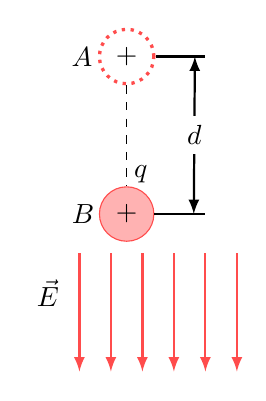
\begin{tikzpicture}
  \node[circle, draw=red!70, very thick, dotted, minimum size=2mm, text=black] (start) at (1,4) {$+$};
  \node[circle, draw=red!70, fill=red!30, minimum size=2mm, text=black] (end) at (1,2) {$+$};
  \draw[dashed] (start) -- (end);
  \draw[thick] (start) -- ++(1,0);
  \draw[thick] (end) -- ++(1,0);
  \draw[thick, latex-latex] ([xshift=5mm]start.east) -- ([xshift=5mm]end.east) node[midway, fill=white] {$d$};
  \node at ([xshift=-2mm]start.west) {$A$};
  \node at ([xshift=-2mm]end.west) {$B$};
  \node at ([xshift=1.8mm,yshift=1.5mm]end.north) {$q$};

  \node at (0, 1) {$\vec{\boldsymbol{E}}$};
	\begin{scope}[xshift=4mm] 
    \foreach \x in {0,1,...,5} {
      \draw[-latex, thick, red!70] (\x*0.4, 1.5) -- (\x*0.4, 0);
    }
	\end{scope}

\end{tikzpicture}
  \caption{A charge $q$ moving in a uniform electric field}
  \label{fig:charge-moving-in-a-uniform-electric-field}
\end{figure}

The potential difference between point $A$ and $B$ is
\begin{equation*}
  \Delta V = V_B - V_A = -\int_A^B \vec{\boldsymbol{E}} \cdot d\vec{\boldsymbol{s}} = -E_0\int_A^B ds = -E_0d < 0
\end{equation*}
Since $-E_0d < 0$, $B$ has a lower electric potential than $A$. The electric field lines indicate where the electric potential is higher, since the lines points from higher potential to lower.

Figure~\ref{fig:potantial-difference-in-a-uniform-electric-field} illustrates the difference in electric potential between two points $A$ and $B$ where they are not parallel to the electric field $\vec{\boldsymbol{E}}$.
\begin{figure}[H]
\centering
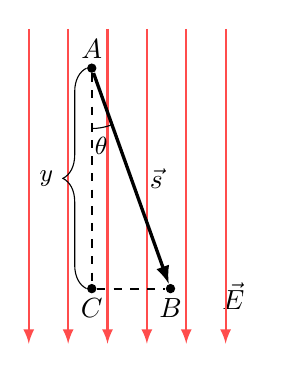
\begin{tikzpicture}

  \node at (3, 0.6) {$\vec{\boldsymbol{E}}$};
	\begin{scope}[xshift=4mm] 
    \foreach \x in {0,1,...,5} {
      \draw[-latex, thick, red!70] (\x*0.5, 4) -- (\x*0.5, 0);
    }
	\end{scope}

  \node[circle, fill, inner sep=1.2pt] (A) at (1.2,3.5) {};
  \node[circle, fill, inner sep=1.2pt] (B) at (2.2,0.7) {};
  \node[circle, fill, inner sep=1.2pt] (C) at (1.2,0.7) {};

  \draw ([yshift=-7mm]A.south) arc[start angle=-90, end angle=-70, radius=7mm] node[midway, below] {\small $\theta$};

  \draw[very thick, -latex] (A) -- (B) node[midway, right=1mm] {$\vec{\boldsymbol{s}}$};
  \draw[thick, dashed] (A) -- (C);
  \draw[thick, dashed] (C) -- (B);

  \node[above] at (A) {$A$};
  \node[below] at (B) {$B$};
  \node[below] at (C) {$C$};

	\draw[decorate, decoration={brace, mirror, amplitude=3mm}] (A.west) -- (C.west) node[midway, left=3mm] {\small $y$};

\end{tikzpicture}
  \caption{Potential difference between two points in a uniform electric field}
  \label{fig:potantial-difference-in-a-uniform-electric-field}
\end{figure}
The difference in electric potential between $C$ and $B$ is zero, since the path is perpendicular to the electric field. Thus, the difference in electric potential does not depend on the angle $\theta$, only the distance between $A$ and $C$, i.e., $y$.

\begin{align*}
  \Delta V &= V_B - V_A = \Delta V_{CA} + \Delta V_{BC} = \Delta V_{CA} \\
  &= -\int_A^B \vec{\boldsymbol{E}} \cdot d\vec{\boldsymbol{s}} = -E_0s\cos{\theta} = -E_0y
\end{align*}


\subsection{Electric Potential due to a Point Charge}
Consider a point charge $Q$. The field produced by $Q$ is $\vec{\boldsymbol{E}}=(Q/4\pi\varepsilon_0r^2)\hat{\boldsymbol{r}}$. From Figure~\ref{fig:potantial-difference-due-to-point-charge} we see that $\hat{\boldsymbol{r}}d\vec{\boldsymbol{s}}=ds\cos{\theta}=dr$. The electric potential difference between two points $A$ and $B$ is therefor
\begin{equation*}
  \Delta V = V_B - V_A = -\int_A^B\frac{Q}{4\pi\varepsilon_0r^2}\hat{\boldsymbol{r}}d\vec{\boldsymbol{s}} = -\int_A^B\frac{Q}{4\pi\varepsilon_0r^2}dr = \frac{Q}{4\pi\varepsilon_0}\left( \frac{1}{r_B} - \frac{1}{r_A} \right)
\end{equation*}

\begin{figure}[H]
\centering
\begin{tikzpicture}

  \coordinate (CQ) at (0, 0);
  \coordinate (CA) at ({sin(-15)*2}, {cos(15)*2});
  \coordinate (CB) at ({sin(70)*4}, {cos(70)*4});
  \coordinate (CR) at ({sin(30)*2.5}, {cos(30)*2.5});

  \node[circle, fill=red!70, inner sep=1.2pt] (Q) at (CQ) {};
  \node[below] at (Q) {$Q$};

  \draw[dashed, blue!30] ([xshift=2cm]Q) arc[start angle=0, end angle=120, radius=2cm];
  \draw[dashed, blue!30] ([xshift=4cm]Q) arc[start angle=0, end angle=120, radius=4cm];

  \node[circle, fill, inner sep=1.2pt] (A) at (CA) {};
  \node[circle, fill, inner sep=1.2pt] (B) at (CB) {};

  \draw[orange!70] (A) to[out=30, in=160] (CR) to[out=-20, in=150] (B);

  \node[above] at (A) {$A$};
  \node[right] at (B) {$B$};

  \draw[thick, -latex] (Q) -- (A) node[midway, left] {$\vec{\boldsymbol{r}}_A$};
  \draw[thick, -latex] (Q) -- (B) node[midway, below] {$\vec{\boldsymbol{r}}_B$};
  \draw[thick, -latex] (Q) -- (CR) node[midway, right] {$\vec{\boldsymbol{r}}$};
  \draw[thick, -latex, blue!60] (CR) -- ($(CR)!0.3!(B)$) node[below] {$d\vec{\boldsymbol{s}}$};
  \draw[thick, -latex, blue!60] (Q) -- ($(Q)!0.3!(CR)$) node[midway, right] {$\hat{\boldsymbol{r}}$};
  \draw[thin] (Q) -- ($(Q)!1.3!(CR)$);
  \draw[thin, dashed] ($(Q)!1.1!(CR)$) -- ($(CR)!0.3!(B)$);

	\draw[decorate, decoration={brace, mirror, amplitude=1mm}] ($(Q)!1.1!(CR)$) -- (CR)  node[near start, left] {\small $dr$};
  \draw ($(CR)!0.07!(B)$) arc[start angle=-20, end angle=70, radius=2mm] coordinate[midway] (midarc); 
  \draw (midarc) -- ++(0.5, 0.2) node[right] {\small $\theta$};
  

\end{tikzpicture}
  \caption{Potential difference between two points due to a point charge.}
  \label{fig:potantial-difference-due-to-point-charge}
\end{figure}


\subsection{Potential Energy in a System of Charges}
Imagine a system of charges is assembled by an external agent. If there is only one charge no work is node $W_1=0$. If the external agent brings a second charge in the system the work done is $W_2=q_2V_1$. Generally the work done is $W_{\text{ext}}=\Delta U$, i.e., the work the external agent has to do is the change in the systems potential energy. For two charges it is
\begin{equation*}
  U_{1\,2} = W_2 = \frac{1}{4\pi\varepsilon_0}\frac{q_1q_2}{r_{1\,2}}
\end{equation*}
And if the external agent brings a third charge the work done for charge $q_3$ is will be
\begin{equation*}
  W_3 = q_3(V_1+V_2)=\frac{q_3}{4\pi\varepsilon_0}\left(\frac{q_1}{r_1\,r_3}+\frac{q_2}{r_{2\,3}}\right)
\end{equation*}
Thus the potential energy is the sum of the all work done
\begin{equation*}
  U = W_2 + W_3 = \frac{1}{4\pi\varepsilon_0}\left(\frac{q_1q_2}{r_{1\,2}}+\frac{q_1q_3}{r_{1\,3}}+\frac{q_2q_3}{r_{2\,3}}\right)
\end{equation*}
The general equation the total potential energy, i.e., work done by the external agent, of $N$ charges is
\begin{equation*}
  U = \frac{1}{4\pi\varepsilon_0} \sum_{i=1}^N\sum_{\substack{j=1 \\ j > i}}\frac{q_iq_j}{r_{i\,j}}
\end{equation*}

\subsection{Deriving Electric Fields from the Electric Potential}
% TODO: deriving electric fields from electric potential
Consider two points separated with a distance $d\vec{\boldsymbol{d}}$, by using Eq.~\ref{eq:electric-potential-difference} we can derive the following differential from:
\begin{equation*}
  dV = -\vec{\boldsymbol{E}}\cdot d\vec{\boldsymbol{s}}
\end{equation*}
In Cartesian coordinates, $\vec{\boldsymbol{E}}=E_x\hat{\boldsymbol{i}}+E_y\hat{\boldsymbol{j}}+E_z\hat{\boldsymbol{k}}$ and $d\vec{\boldsymbol{s}}=dx\hat{\boldsymbol{i}}+dy\hat{\boldsymbol{j}}+dz\hat{\boldsymbol{k}}$, we have
\begin{equation*}
  dV = \left(E_x\hat{\boldsymbol{i}}+E_y\hat{\boldsymbol{j}}+E_z\hat{\boldsymbol{k}}\right)\cdot\left(dx\hat{\boldsymbol{i}}+dy\hat{\boldsymbol{j}}+dz\hat{\boldsymbol{k}}\right) = E_xdx + E_ydy + E_zdz
\end{equation*}
which implies
\begin{equation*}
  E_x = -\frac{\partial V}{\partial x},\: E_y = -\frac{\partial V}{\partial y},\: E_z = -\frac{\partial V}{\partial z}
\end{equation*}
We now introduce a differential quantity called the ``del (gradient) operator'' to simplifiy the notation.
\begin{equation*}
  \nabla \equiv \frac{\partial}{\partial x} \hat{\boldsymbol{i}} + \frac{\partial}{\partial y} \hat{\boldsymbol{j}} + \frac{\partial}{\partial z} \hat{\boldsymbol{k}} 
\end{equation*}
We then get 
\begin{equation*}
  \vec{\boldsymbol{E}} =  E_x\hat{\boldsymbol{i}} + E_y\hat{\boldsymbol{j}} + E_z\hat{\boldsymbol{k}}
-\left(\frac{\partial V}{\partial x} \hat{\boldsymbol{i}} + \frac{\partial V}{\partial y} \hat{\boldsymbol{j}} + \frac{\partial V}{\partial z} \hat{\boldsymbol{k}}\right)
  = 
  \left(\frac{\partial}{\partial x} \hat{\boldsymbol{i}} + \frac{\partial}{\partial y} \hat{\boldsymbol{j}} + \frac{\partial}{\partial z} \hat{\boldsymbol{k}}\right)V = -\nabla V
\end{equation*}

\begin{equation}\label{eq:electric-field-del-gradient-potential}
  \vec{\boldsymbol{E}} = -\nabla V
\end{equation}

If the charges in the system is having a spherical electric field, the electric field is a function of the radial distance $r$, i.e., $\vec{\boldsymbol{E_r}}=E_r\hat{\boldsymbol{r}}$, when $dV = -E_r dr$. If $V(r)$ the electric field can then be obtained
\begin{equation*}
  \vec{\boldsymbol{E}} = E_r\hat{\boldsymbol{r}} = -\left( \frac{dV}{dr} \right)\hat{\boldsymbol{r}}
\end{equation*}
For instance, electric potential due to a point charge's electric field can be calculated as $V(r)=q/4\pi\varepsilon_0 r$. Thus, the electric field produced is $\vec{\boldsymbol{E}}=(q/4\pi\varepsilon_0 r^2)\hat{\boldsymbol{r}}$.



\subsection{Gradient and Equipotentials}
% TODO: Graidiant and endpoints
%Eq.~\ref{eq:electric-field-del-gradient-potential}

An equipotential curve shows the levels of electric potential. The intersection of the equipotential curve and the electric field lines are always perpendicular, i.e., $\vec{\boldsymbol{E}} \perp d\vec{\boldsymbol{s}}$, shown in Figure~\ref{fig:equipotential-curves-and-electric-field-lines}. The difference in the electric potential between two levels of the equipotential curve is 
\begin{equation*}
  dV = \left( \frac{\partial V}{\partial x}\hat{\boldsymbol{i}} + \frac{\partial V}{\partial y}\hat{\boldsymbol{j}} \right)\cdot\left( dx\hat{\boldsymbol{i}} + dy\hat{\boldsymbol{j}} \right) = (\nabla)\cdot d\vec{\boldsymbol{s}} = -\vec{\boldsymbol{E}}\cdot d\vec{\boldsymbol{s}}
\end{equation*}

% Perpendicular
% Equipotetial cuervs


\begin{figure}[H]
\centering
\begin{subfigure}[b]{0.3\textwidth}
  \centering
\begin{tikzpicture}
  \foreach \d in {0,0.5,...,3.5} {
    \draw[red!70, -Stealth] (-0.2,\d) -- (3.8,\d);
    \draw[blue!60, dashed] (\d,-0.2) -- (\d,3.8);
  }
  \node at (4.1,3.3) {$\vec{\boldsymbol{E}}$};
\end{tikzpicture}
  \caption{} 
  %\label{fig:electric-field-line-for-positive} 
\end{subfigure}
    \hfill
\begin{subfigure}[b]{0.26\textwidth}
  \centering
\begin{tikzpicture}[
      scale=0.70,
      attach arrow/.style args={#1}{
          decoration={
              markings,
              mark=at position 0 with {\pgfextra{%
                  \pgfmathsetmacro{\tmpArrowTime}{\pgfkeysvalueof{/tikz/arc arrow/length}/(\pgfdecoratedpathlength)}%
                  \xdef\tmpArrowTime{\tmpArrowTime}}},
              mark=at position {#1-3*\tmpArrowTime} with {\coordinate(@1);},
              mark=at position {#1-2*\tmpArrowTime} with {\coordinate(@2);},
              mark=at position {#1-1*\tmpArrowTime} with {\coordinate(@3);},
              mark=at position {#1+\tmpArrowTime/2} with {\coordinate(@4);
                  \draw[-{Stealth[length=\pgfkeysvalueof{/tikz/arc arrow/length},bend]}]
                    plot[smooth] coordinates {(@1) (@2) (@3) (@4)};},
          },
          postaction=decorate,
      },
      attach arrow/.default=0.5,
      arc arrow/.cd, length/.initial=2mm,
  ]
  \node[draw=red!70, fill=red!30, circle, minimum size=6mm] (Q) {$+$};
  
  % Radial inward field lines
  \foreach \a in {0,30,...,330} {
    \draw[red!70, thick, attach arrow={1/2}] (Q) -- ++(\a:3);
  }
  \draw[blue!60, dashed] (L) circle (8mm);
  \draw[blue!60, dashed] (L) circle (14mm);
  \draw[blue!60, dashed] (L) circle (24mm);
\end{tikzpicture}
  \caption{}
  %\label{fig:electric-field-line-for-positive}
\end{subfigure}
    \hfill
\begin{subfigure}[b]{0.4\textwidth}
    \centering
\begin{tikzpicture}[
    scale=0.7,
    attach arrow/.style={
        decoration={
            markings,
            mark=at position 0 with {\pgfextra{%
                \pgfmathsetmacro{\tmpArrowTime}{\pgfkeysvalueof{/tikz/arc arrow/length}/(\pgfdecoratedpathlength)}%
                \xdef\tmpArrowTime{\tmpArrowTime}}},
            mark=at position {#1-3*\tmpArrowTime} with {\coordinate(@1);},
            mark=at position {#1-2*\tmpArrowTime} with {\coordinate(@2);},
            mark=at position {#1-1*\tmpArrowTime} with {\coordinate(@3);},
            mark=at position {#1+\tmpArrowTime/2} with {\coordinate(@4);
                \draw[-{Stealth[length=\pgfkeysvalueof{/tikz/arc arrow/length},bend]}] plot[smooth]
                coordinates {(@1) (@2) (@3) (@4)};},
        },
        postaction=decorate,
    },
    attach arrow/.default=0.5,
    arc arrow/.cd,length/.initial=2mm,
    %nodes={circle,minimum size=2.4em,font=\bfseries\sffamily}
]
  \path 
      node[draw=red!70, fill=red!30, circle, minimum size=4mm] (L){$+$} 
      (2.5,0) node[draw=blue!60, fill=blue!10, circle, minimum size=4mm] (R){$-$};
  \foreach \X in {0,...,4}
   {\draw[red!70, thick, attach arrow] (L) 
   to[bend left={-70+\X*35},looseness=1.6] 
   (R);}
  \foreach \X in {0,...,5}
   {\draw[red!70, thick,attach arrow/.list={1/2}] (L) to[bend left=16-8*\X] ++ (70+\X*44:3);
   \draw[red!70, thick,attach arrow/.list={1/2}] (R)+(180+70+\X*44:3) 
   to[bend right=16-8*\X] 
    (R);}
  \draw[blue!60, dashed] (L) ellipse (8mm and 7mm);
  \draw[blue!60, dashed] ([xshift=-1.4mm]L) ellipse (10mm and 9.5mm);
  \draw[blue!60, dashed] ([xshift=-3.6mm]L) circle (14mm);
  \draw[blue!60, dashed] ([xshift=-8.2mm]L) circle (20mm);
  \draw[blue!60, dashed] (1.2,-3) -- (1.2,3);
  \draw[blue!60, dashed] (R) ellipse (8mm and 7mm);
  \draw[blue!60, dashed] ([xshift=1.4mm]R) ellipse (10mm and 9.5mm);
  \draw[blue!60, dashed] ([xshift=3.6mm]R) circle (14mm);
  \draw[blue!60, dashed] ([xshift=8.2mm]R) circle (20mm);
\end{tikzpicture}
  \caption{}
  %\label{fig:electric-field-line-negative}
  \end{subfigure}
  \caption{A charge $q$ moving in a constant electric field formed by two infinity large source plates.}
  \label{fig:equipotential-curves-and-electric-field-lines}
\end{figure}





\section{Gauss' Law}
\section{Capacitors}
\section{Current and Resistance}
\section{Direct Current Circuits}
\section{Magnetic Fields}
\section{Sources of Magnetic Fields}
\section{Faraday's Law}
\section{Inductance and Energy in Magnetic Fields}
\section{Alternating Current Circuits}
\section{Maxwell's Equations and Electromagnetic Waves}
\section{Interference and Diffraction}


